\documentclass[12pt, a4paper]{article}
\usepackage[francais]{babel}
\usepackage{caption}
\usepackage{graphicx}
\usepackage[T1]{fontenc}
\usepackage{listings}
\usepackage{geometry}
\usepackage{minted}
\usepackage{array,multirow,makecell}
\setcellgapes{1pt}
\makegapedcells


\renewcommand{\listingscaption}{Code}

\begin{document}
    \title{\huge SAE 23 - Mettre en place une
    solution informatique pour l'entreprise \\[5cm] \Large \medskip Fiche de procédure des parties importantes de la mise en place de notre application}
    \author{\\[2cm]Martin Baumgaertner}
    \date{\today}
    \maketitle
    \maketitle
    \newpage
    \tableofcontents
    \newpage
    \section{Introduction}
    Pour pouvoir mettre à bien notre SAE, il va falloir d’abord comprendre ce que le sujet veut nous faire comprendre. Nous devons réaliser une interface graphique sur l’internet qui permet la gestion de notes. 
    Nous possèdons plusieurs domaines que nous devons relier à des sous-domaines. Je vais les lister ci-après sous forme de tableau :\\[0.5cm]
    \begin{tabular}{|l|l|}
        \hline
        \multirow{6}{*}{Étudiant} 
          & Numéro étudiant \\
          & Nom \\
          & Prénom \\
          & Groupe \\
          & Photo \\
          & E-mail \\ \hline
        \multirow{4}{*}{Unité d'enseignement}
          & Code \\
          & Nom \\
          & Semestre \\
          & ECTS \\ \hline
        \multirow{4}{*}{Resource associé aux UEs} 
          & Code ressource \\
          & Nom \\
          & Descriptif \\
          & Coefficient \\ \hline
        \multirow{2}{*}{Enseignants} 
          & Nom \\
          & Prénom \\ \hline
        \multirow{4}{*}{Examens} 
          & ID \\
          & Titre \\
          & Date \\
          & Coefficient \\ \hline
        \multirow{4}{*}{Notes} 
          & Examen \\
          & Étudiant \\
          & Note \\
          & Appréciation \\ \hline
      \end{tabular}
        \newpage
        \subsection{Création de la base de données}
        J’ai donc créé la base de données comme demandé à partir de TablePlus, un éditeur/créateur de base de données. J’ai choisi d’utiliser TablePlus pour sa facilité d’utilisation et son design innovateur. On comprend rapidement comment utiliser l’éditeur à l’inverse de phpMyAdmin par exemple. 
        J’ai créé les tables en veillant à ajouter les bonnes clés étrangères et les bons paramètres. Voici les tables créees : \\[0.5cm]
        \begin{figure}[h]
            \centering
            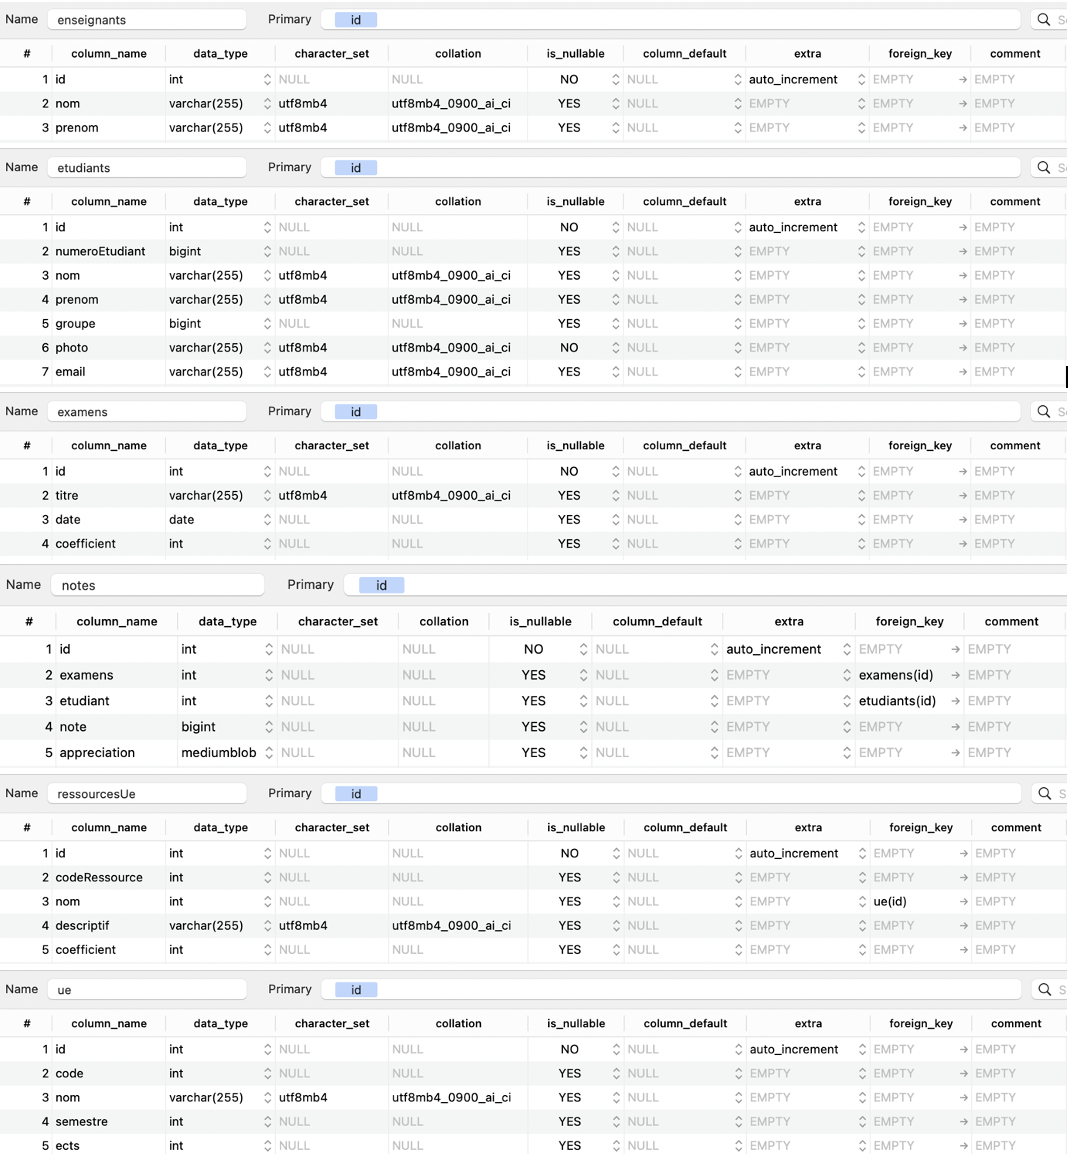
\includegraphics[width=0.8\textwidth]{img1.png}
            \caption{Base de données}
            \label{fig:basededonnees}
        \end{figure}
        \newpage
        \subsection{Import de la base de données dans Django}
        Pour commencer, il faut donc lier notre base de données, pour ce faire nous devons éditer notre fichier settings.py dans les paramètres « database » :
        \begin{listing}[H]
            \caption{code settings.py}
            \label{lst:settings}
            \begin{minted}{python}
                DATABASES = {
                    'default': {
                    'ENGINE': 'django.db.backends.mysql',
                    'NAME': 'grade', 
                    'USER': 'root',
                    'HOST': 'localhost',
                    'PORT': '3306',
                    'PASSWORD': 'webgradedatabase',
                    }
                }
            \end{minted}
        \end{listing}
        Ensuite j’ai donc pu connecter ma base de données à mon projet Django. 
        \\J’ai fait la commande « python3 manage.py makemigrations » pour pouvoir faire les migrations, puis je les ai appliqués avec la commande «python3 manage.py migrate » :
        \\[1cm]Par la suite, j'ai voulu donc crée un fichier models.py à partir de la base de données que je viens de créer en SQL :
        \begin{minted}{bash}
            python3 manage.py inspectdb > models.py
        \end{minted}
        Suite à cela j'ai donc bien obtenu mon fichier models.py avec toutes les "class" qui ont bien été créees.
    \newpage
    \section{Développement Backend}
        \subsection{Gestion des CRUDs}
            \subsubsection{Démarrage de la création des CRUDs}
            Après avoir donc récupéré mes différents « models » j’ai pu commencer le développement de la partie backend. J’ai configuré mes vues, mes templates pour obtenir d’abord des formulaires fonctionnels pour tous les CRUDs. Ensuite j’ai directement créé un .html squelette car je me suis vite rendu compte que j’allais avoir besoin de beaucoup de fichier html. J’ai mis dedans une barre de recherche qui relie tous les formulaires et les liens importants. 
            \\[0.5cm]Pour pouvoir ajouter des images aux élèves il a fallu au préalable bien éditer la base de données. Au début mon champ image dans MySQL était de type « blob » car je pensais que c’était le paramètre adéquat. Mais en fin de compte lorsque je voulais récupérer les images pour les afficher, j’avais le chemin de destination de l’image qui s’affichait et non pas l’image. Donc après plusieurs recherches je me suis rendu compte que le bon paramètre MySQL pour les images était de type « Varchar ». 
            En plus de cela il nous faut ajouter dans le fichier « settings.py » ces lignes de code :
            \begin{listing}[h]
                \caption{code settings.py}
                \label{lst:static}
                \begin{minted}{python}

                STATIC_URL = '/static/'
                MEDIA_URL = '/media/'

                MEDIA_ROOT = os.path.join(BASE_DIR, 'media/')

                STATICFILES_DIRS = (
                    os.path.join(BASE_DIR, 'static'),
                )
                \end{minted}
            \end{listing}
            \newpage
            On indique ici à notre projet d’aller chercher dans le fichier /media pour retrouver les images. 
            Puis, dans le fichier « urls.py » de notre projet on va venir rajouter à la fin que nous voulons ajouter la possibilité de pouvoir charger des images :
            \begin{figure}[h]
                \centering
                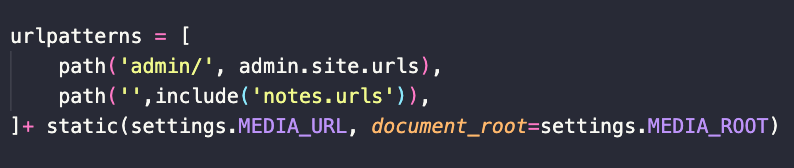
\includegraphics[width=0.9\textwidth]{url.png}
                \caption{Code URL du projet}
                \label{fig:url}
            \end{figure}
            \\Après avoir correctement éditer notre fichier « views.py » en demandant bien à notre fonction de récupérer les images comme ici : 
            \begin{minted}{python}
            form = EtudiantsForm(request.POST, request.FILES)
            \end{minted}
            Nous avons notre projet qui fonctionne avec des images.
        \subsection{Fonction recherche étudiant}
            \subsubsection{Views.py}
            Nous devons premièrement créer une vue dans notre fichier views.py qui consistera à dire que si l’on recherche un étudiant depuis un prénom, views.py ira chercher dans notre fichier models.py tous les prénoms des étudiants matchant avec notre recherche. S’il y a des résultats à afficher, alors, les résultats iront dans la variable « etudiants » pour qu’on puisse afficher les résultats dans une page html. Voici donc ci-dessous ce que j’ai développé pour avoir la fonction recherche fonctionnelle. 
            \begin{figure}[h]
                \centering
                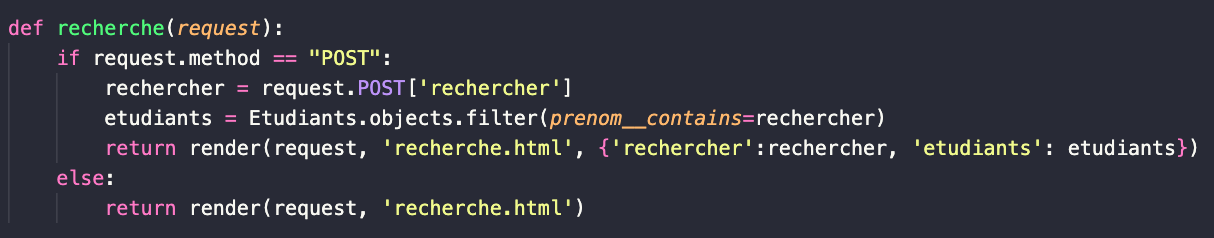
\includegraphics[width=1\textwidth]{recherche.png}
                \caption{Code du fichier Views.py}
                \label{fig:recherche}
            \end{figure}
            \newpage
            \subsubsection{html}
            Pour pouvoir afficher les valeurs que nous retourne notre vue, il faut donc créer un fichier html. Dedans on va donc définir que s’il y a une recherche AVEC résultat, nous irons rechercher parmi tous les étudiants le nom et l’étudiant ainsi que son prénom. Et, si la recherche est vide et qu’on ne recherche rien, un texte disant « vous n’avez pas recherché » apparaît chez l’utilisateur. 
            \begin{figure}[h]
                \centering
                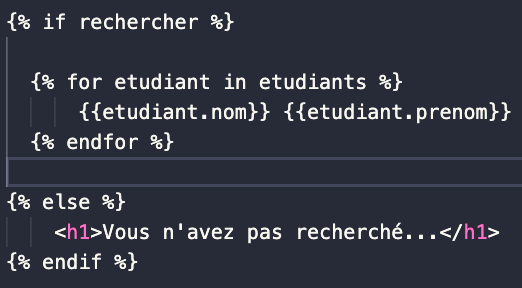
\includegraphics[width=0.8\textwidth]{html.png}
                \caption{Code HTML}
                \label{fig:html}
            \end{figure}
    \newpage
    \section{Mise en place de notre application sur serveur linux}    
        \subsection{Configuration de la machine}
            \subsubsection{Installation de base}
            Pour commencer, j’ai choisi de mettre en place mon serveur sur une machine sous Debian11, je l’ai installé en mode console uniquement. Puis, j’ai récupéré mon projet depuis GitHub en effectuant la commande « git clone https://martinbaumg/SAE-23 ». 
            \subsubsection{Création de l'environnement virtuel}
            Une fois fait j’ai créé un environnement virtuel que j’ai nommé « venv » 
            Dans cet environnement virtuel j’ai installé pour les prérequis pour l’application, donc Django, Pip, et Pillow qui sert à la mise en place des éléments photos. 
        \subsection{Mise en place de la base de données}
        Pour mettre en place la base de données j’ai installé MariaDB-server et client ainsi que MySQL. J’ai exporté la base de données que j’avais créé sur ma machine hôte et je l’ai transféré sur ma machine Debian. Ensuite, j’ai donc ouvert MariaDB et créée une base de données que j’ai nommé « grade » à l’aide de la commande suivante : 
        \begin{minted}{sql}
            CREATE DATABASE grade;
        \end{minted}
        Puis, j’ai importé ma base de données déjà existante dans la nouvelle base de données que je viens de créer dans MariaDB avec cette commande, depuis le terminal linux : 
        \begin{minted}{sql}
            mysql -u root -p grade < grade.sql 
        \end{minted}
        \newpage
        \subsection{Modification du fichier settings.py}
            \subsubsection{Adresse IP}
            J’ai modifié certains champs du fichier settings du projet pour que tout fonctionne, premièrement, cette ligne, dans laquelle j’ai ajouté mon adresse IP : 
            \begin{listing}[H]
                \caption{Adresse IP}
                \label{lst:ip}
                \begin{minted}{python}
                    ALLOWED_HOSTS = ['192.168.64.6']
                \end{minted}
            \end{listing}
            \subsubsection{Base de données}
            Pour pouvoir mettre en place la base de données avec le projet j’ai dû me connecter à la base de données que j’ai créée avec MariaDB, pour ce faire j’ai créé un utilisateur depuis MariaDB, et je lui ai donnée tous les droits, à l’aide des commandes suivantes :
            \begin{listing}[H]
                \caption{code sql}
                \label{lst:sql}
                \begin{minted}{sql}
                CREATE USER 'django'@'localhost' IDENTIFIED BY 'password';
                GRANT ALL PRIVILEGES ON grade.* TO  'django'@'localhost';
                \end{minted}
            \end{listing}
            \subsubsection{Deployment de l'application}
            J’ai donc fait la commande « python3 manage.py runserver 0.0.0.0:8000 ». 
            \\On indique à notre serveur de démarrer le projet sur l’adresse IP de la machine sur le port 8000.
            Enfin, en écrivant donc l’adresse IP de la machine suivis du port 8000 nous retrouvons donc localement sur notre machine l’application. 
            \begin{figure}[h]
                \centering
                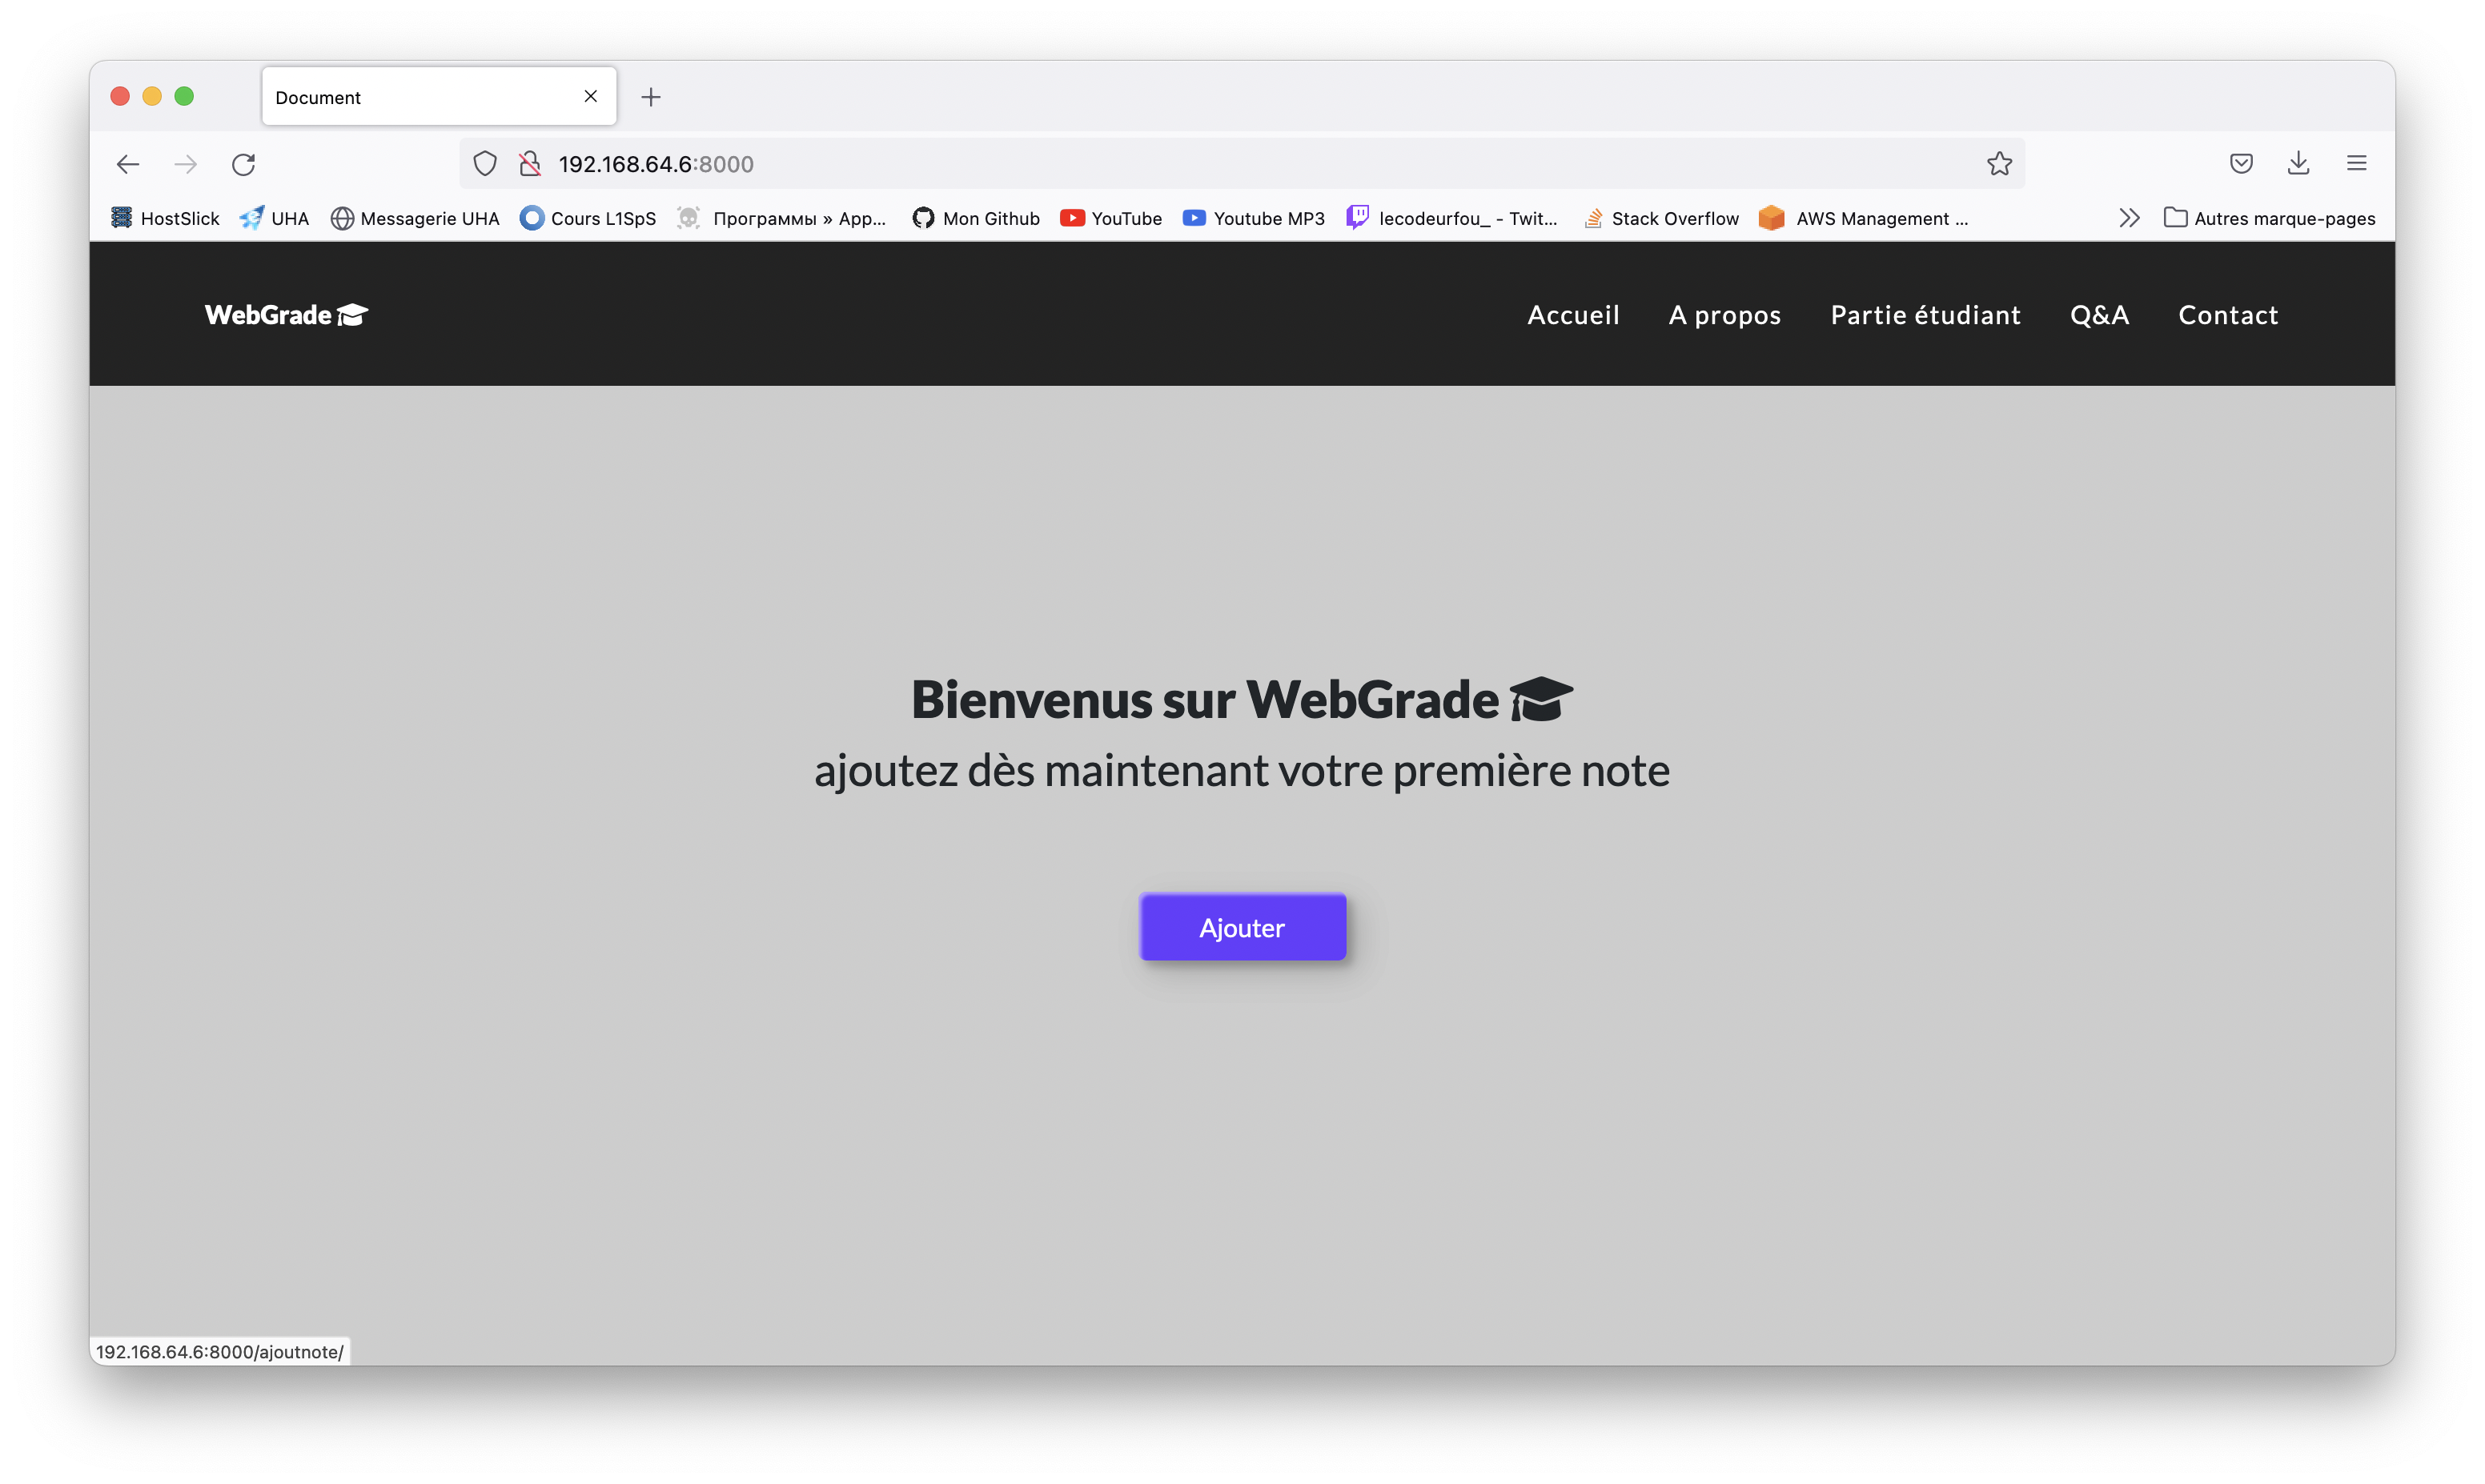
\includegraphics[width=0.9\textwidth]{dep.png}
                \caption{Notre application deployée}
                \label{fig:dep}
            \end{figure}

            

              
              
            

\end{document}